\documentclass[titlepage,a4paper]{article}

\usepackage[utf8]{inputenc} % ensures input is UTF-8
\usepackage[landscape]{geometry}

\usepackage{tikz}
\usetikzlibrary{arrows,automata,positioning}

\begin{document}

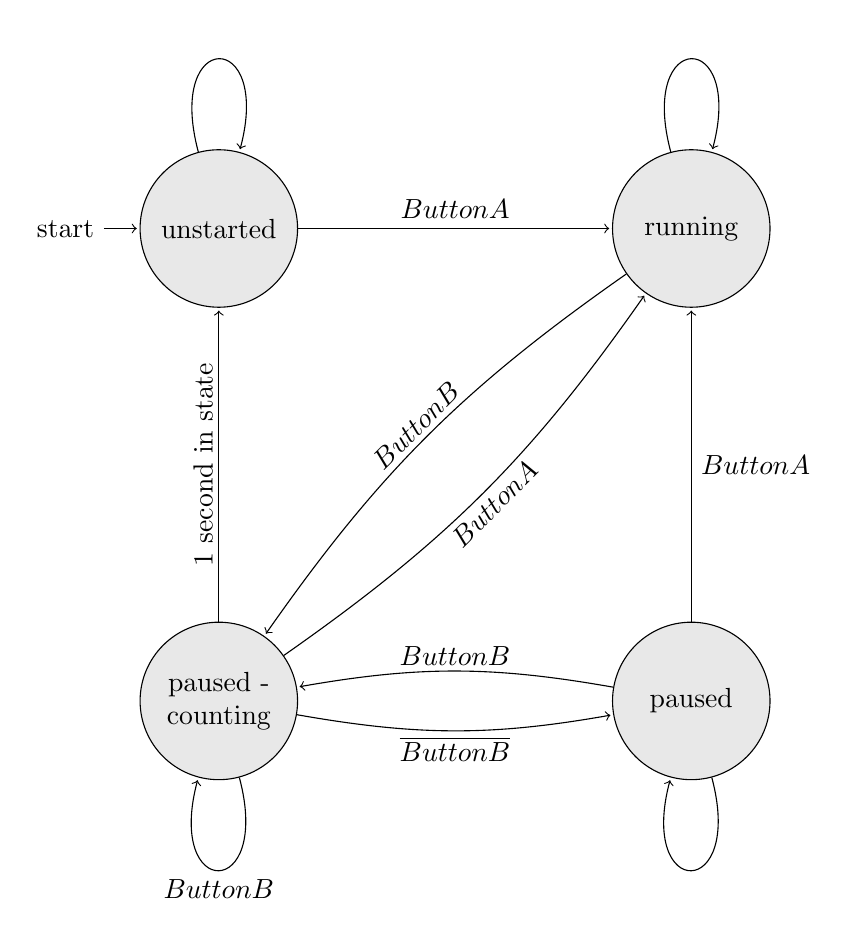
\begin{tikzpicture}[shorten >=1pt,
    node distance=6cm,
    auto,
    every text node part/.style={align=center},
    el/.style = {inner sep=2pt, align=left, sloped}
  ]
  \tikzstyle{every state}=[fill={rgb:black,1;white,10},minimum size=2cm,text width=1.5cm]

  \node[state,initial]  (s_1)                    {unstarted};
  \node[state]          (s_2)  [right of=s_1]    {running};
  \node[state]          (s_3)  [below of=s_1]    {paused - counting};
  \node[state]          (s_4)  [right of=s_3]    {paused};

  \path[->]
  (s_1) edge [loop above]    node []          {}                      (   )
        edge                 node []          {$Button A$}            (s_2)
  (s_2) edge [bend right=10] node [el, above] {$Button B$}            (s_3)
        edge [loop above]    node []          {}                      (   )
  (s_3) edge [loop below]    node []          {$Button B$}            (   )
        edge [bend right=10] node [el, below] {$\overline{Button B}$} (s_4)
        edge [bend left=-10] node [el, below] {$Button A$}            (s_2)
        edge                 node [el, above] {1 second in state}            (s_1)
  (s_4) edge [loop below]    node []          {}                      (   )
        edge [bend left=-10] node [el, above] {$Button B$}            (s_3)
        edge                 node [right]     {$Button A$}            (s_2)
  ;
\end{tikzpicture}

\end{document}
